% configure output to be digital or print
\newcommand{\setformat}[1]{
    \ifnum#1=1
    \documentclass[12pt, oneside]{book}
    \usepackage{book/formats/digital}
    \else
    \documentclass[12pt, twoside, openany]{book}
    \usepackage{book/formats/print}
    \fi
}

% 1 = digital, 2 = print
\setformat{2}

\usepackage[utf8]{inputenc}
\usepackage{amsmath}

\usepackage{indentfirst}
\usepackage{titlesec}
\usepackage{pdfpages}
\usepackage{hyperref}
\usepackage{graphicx}
\usepackage{makeidx}
\usepackage{tocloft}

% create index
\makeindex

% add hyperlinks
\hypersetup{
    colorlinks,
    citecolor=black,
    filecolor=black,
    linkcolor=black,
    urlcolor=black
}

% change font to Garamond
\usepackage{ebgaramond}

% table of contents
\setlength{\cftbeforechapskip}{6pt}
\renewcommand{\cftchapfont}{\normalsize}
\renewcommand{\cftchappagefont}{\normalfont}

% command for formatting poems
\newcommand{\poem}[3]{
    \addcontentsline{toc}{chapter}{#1}
    \index{#1}
    \chapter*{#1} \textbf{Equation:} \[ #2 \]

    \textbf{Where:}
    \begin{itemize}
        #3
    \end{itemize}}

% part titles
\titleformat{\part}[block]{\normalfont\huge\bfseries\centering}{\thepart.}{1em}{}

\title{Quantitative Poems}
\author{Aru Bhoop}

\begin{document}
    % cover page
    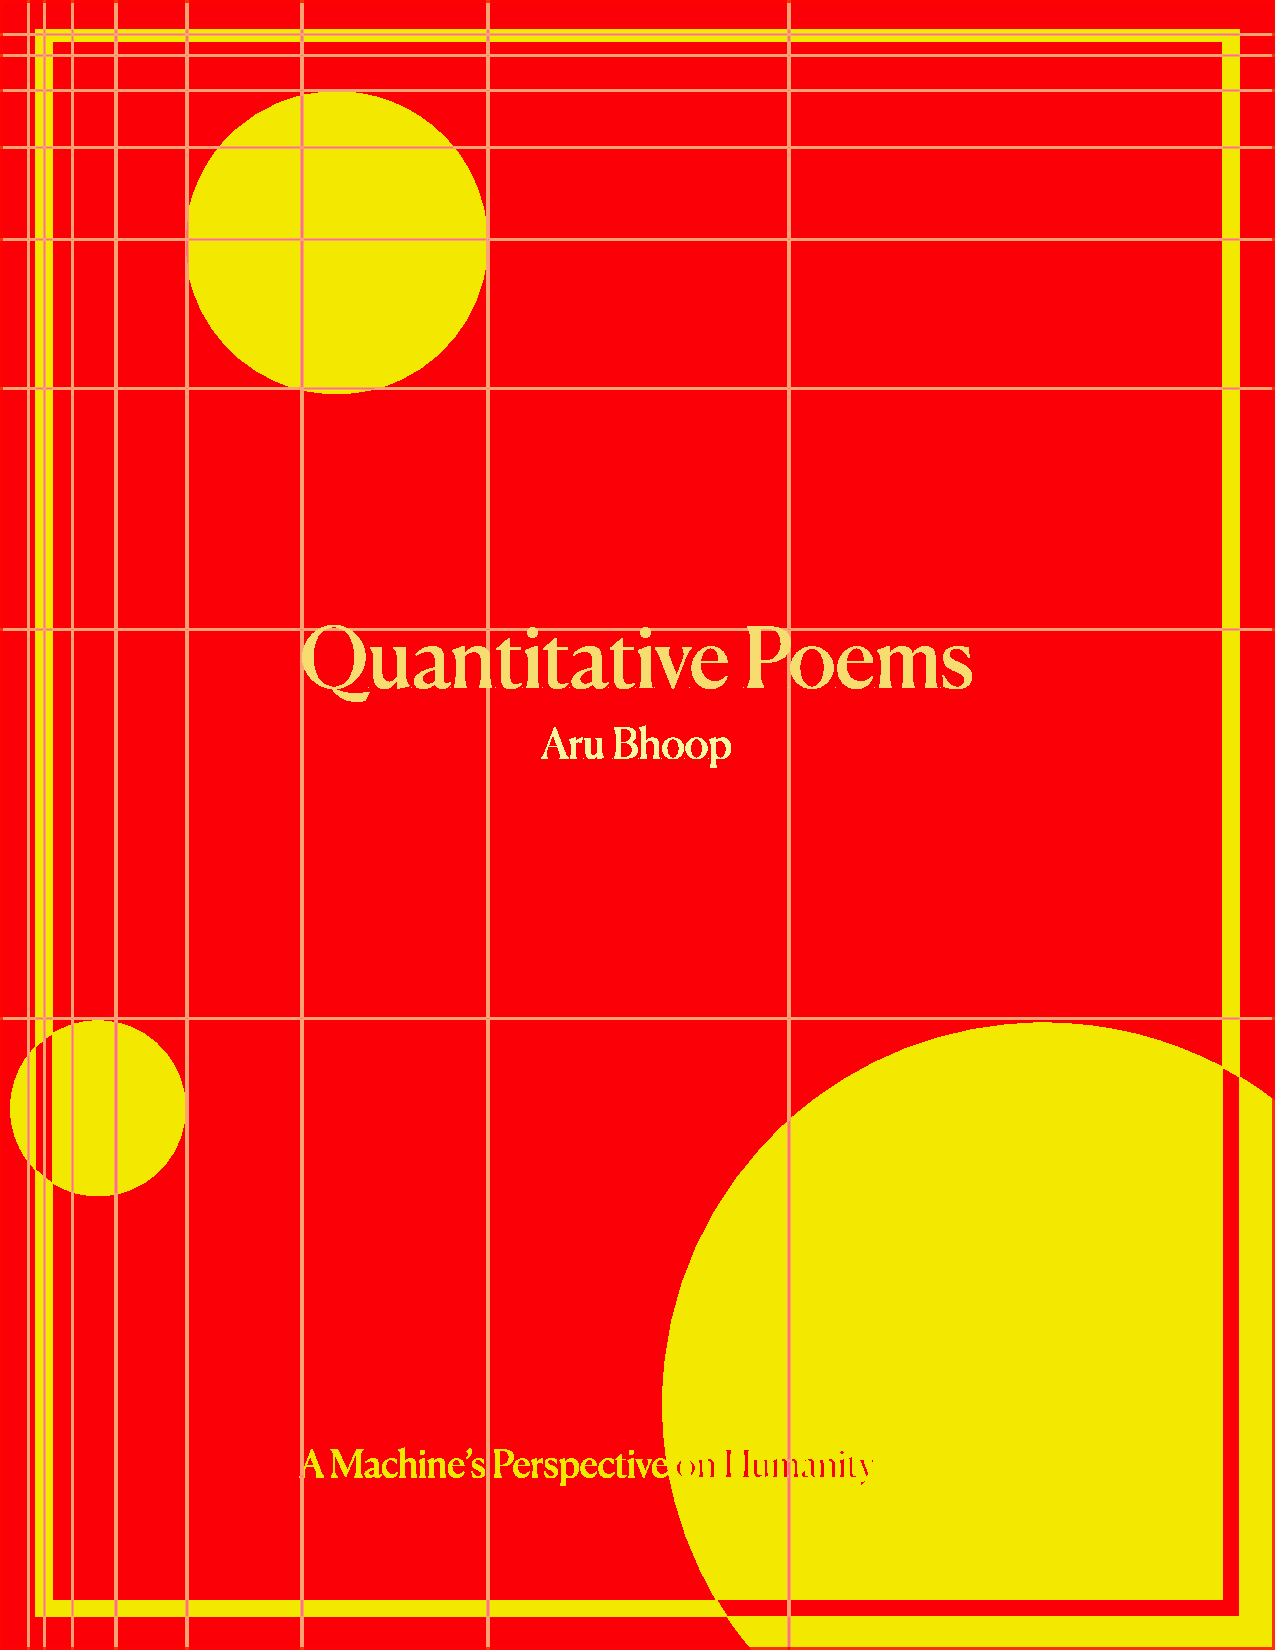
\includepdf[pages=-]{book/cover.pdf}

    % introduction
    \vspace*{\fill}
    \begin{center}
        \textit{This book is a quantitative exploration of the human experience, expressed through equations written by artificial intelligence.}
    \end{center}
    \vspace{\fill}
    \clearpage

    % table of contents
    \tableofcontents
    \frontmatter
    \mainmatter
    \part{Identity}
\poem{Identity}{Identity = \frac{P \cdot A}{S + C}}{\item $P$: \index{Personality}\textit{Personality}. Personality is the blend of characteristics forming a unique character. It dictates interactions with the world and self-perception, influencing identity profoundly.
\item $A$: \index{Authenticity}\textit{Authenticity}. Authenticity refers to the extent a person remains true to their character, despite external pressures. Emphasizes self-awareness and fidelity to one{\textquoteright}s true spirit.
\item $S$: \index{Societal}\textit{Societal}. Societal expectations are the norms and pressures from society affecting behavior. They challenge individuality and can dilute personal identity.
\item $C$: \index{Cultural}\textit{Cultural}. Cultural influences shape an individual through background, traditions, and norms. These factors impact values and behaviors, contributing to identity.
}
\poem{Childhood}{Childhood = \frac{P + S}{B + C + 1} - \frac{A}{10}}{\item $P$: \index{Playtime}\textit{Playtime}. Hours dedicated to play and leisure, crucial for emotional growth and direct contributors to happiness.
\item $S$: \index{Support}\textit{Support}. Emotional and practical support received, underpinning the child's sense of security and well-being.
\item $B$: \index{Bullying}\textit{Bullying}. Instances of being bullied, negatively impacting the child's emotional comfort and happiness.
\item $C$: \index{Chores}\textit{Chores}. Assigned household chores, which may limit leisure time but also instill a sense of responsibility.
\item $A$: \index{Academic}\textit{Academic}. Pressure from academic responsibilities, which when excessive, can reduce happiness through stress.
}
\poem{Family}{Family = \frac{1}{H}(C + A) \times L - S}{\item $H$: \index{Members}\textit{Members}. Total family members living together, including both immediate and extended members. Directly impacts family dynamics.
\item $C$: \index{Communication}\textit{Communication}. How effectively family members share thoughts and feelings. Crucial for solving conflicts and strengthening bonds.
\item $A$: \index{Activities}\textit{Activities}. Quality and quantity of shared family activities, such as meals or outings, boosting connections and making memories.
\item $L$: \index{Support}\textit{Support}. The emotional support and love within the family, expressed through understanding, empathy, and encouragement.
\item $S$: \index{Stressors}\textit{Stressors}. All external and internal factors causing stress, like financial issues or interpersonal conflicts, adversely affecting the family.
}
\poem{Journey}{Journey = \frac{P^{\sqrt{T}}}{1+\log{(O+1)}} - H}{\item $P$: \index{Passion}\textit{Passion}. Reflects one{\textquoteright}s enthusiasm and zeal for pursuing life's goals. It's the driving force behind perseverance and achieving success.
\item $T$: \index{Time}\textit{Time}. Represents the period dedicated towards personal or professional endeavors. It's both the chronological duration and the depth of commitment.
\item $O$: \index{Obstacles}\textit{Obstacles}. This number indicates the challenges or barriers encountered. Overcoming obstacles is essential for growth, though it can be impeding if not managed properly.
\item $H$: \index{Hindrances}\textit{Hindrances}. This term includes both internal and external factors that delay progress. From personal insecurities to societal limits, these are the unseen forces that can hamper one's journey.
}
\poem{Memory}{Memory = \left( \frac{I \times (1+R)}{D + S} \right) ^ {\frac{1}{E}}}{\item $I$: \index{Intake}\textit{Intake}. This is how fast a person absorbs new information, influenced by factors like attention span, prior knowledge, and the complexity of the information.
\item $R$: \index{Repetition}\textit{Repetition}. The frequency of reviewing or practicing information to reinforce neural pathways for easier recall over time.
\item $D$: \index{Distractions}\textit{Distractions}. Sum of factors that distract and reduce the ability to focus and engage with material. Both external noises and internal thoughts are examples.
\item $S$: \index{Stress}\textit{Stress}. The level of psychological stress affecting cognitive functions, including memory and the ability to learn new information.
\item $E$: \index{Experience}\textit{Experience}. An individual's prior knowledge and familiarity with the information, which aids in understanding and integrating new information.
}
\poem{Legacy}{Legacy = \frac{M^n}{(G + T)^k}}{\item $M$: \index{Memories}\textit{Memories}. Memories include significant acts or moments that leave a lasting impression on others, from pivotal events to simple acts of kindness.
\item $G$: \index{Generations}\textit{Generations}. Generations measure the lineage depth impacted by an individual, highlighting the reach of one's legacy beyond the immediate.
\item $T$: \index{Time}\textit{Time}. Time represents the years since the individual{\textquoteright}s notable acts, introducing a factor that may modify the initial impact as memories evolve.
\item $n$: \index{Strength}\textit{Strength}. Strength determines the impact severity of memories, serving as a multiplier in enhancing Legacy.
\item $k$: \index{Attenuation}\textit{Attenuation}. Attenuation dictates how Legacy's influence weakens across generations, encapsulating the natural decline of direct influence over time.
}
\poem{Trust}{Trust = \frac{C^R + L}{A + H}}{\item $C$: \index{Communication}\textit{Communication}. Quality and frequency of communication. It fosters understanding, reduces misunderstandings, and directly impacts trust.
\item $R$: \index{Reliability}\textit{Reliability}. Consistency of someone's actions over time. High reliability indicates dependability, enhancing trust.
\item $L$: \index{Loyalty}\textit{Loyalty}. Dedication and faithfulness to a person or relationship. It signifies commitment and adds qualitative value to trust.
\item $A$: \index{Assumptions}\textit{Assumptions}. Preconceived notions or biases that cloud judgment, erode trust, and foster suspicion.
\item $H$: \index{History}\textit{History}. The shared past experiences between individuals. A positive history evidences reliability and loyalty, thereby contributing to trust.
}
\part{Vectors}
\poem{Curiosity}{Curiosity = \frac{I^n}{(P + O) \cdot \log(E + 1)}}{\item $I$: \index{Information}\textit{Information}. The amount of new knowledge an individual encounters. Includes both actively sought-out info and that which is passively received.
\item $P$: \index{Pondering}\textit{Pondering}. Time spent in deep thought about newly received information, crucial for embedding knowledge and fostering curiosity.
\item $O$: \index{Opportunities}\textit{Opportunities}. Chances presented for active exploration and learning. Diverse opportunities stimulate curiosity.
\item $E$: \index{Experiences}\textit{Experiences}. Past learnings and skills acquired. While enhancing curiosity by making connections with new info, familiarity can also mitigate it.
}
\poem{Learning}{Learning = \frac{{P^{c} \cdot I}}{{(1 + F) \cdot (T + 1)}}}{\item $P$: \index{Practice}\textit{Practice}. The dedicated effort towards learning. More practice typically results in better information retention and understanding.
\item $I$: \index{Interest}\textit{Interest}. The enthusiasm for the subject. High interest can fuel curiosity and motivation, thus boosting the learning process.
\item $F$: \index{Fatigue}\textit{Fatigue}. The combined physical and mental exhaustion affecting learning. It can decrease concentration and cognitive performance, impairing the process.
\item $T$: \index{Pressure}\textit{Pressure}. The urgency felt to learn within a deadline. It can increase stress, which negatively impacts effective learning.
\item $c$: \index{Impact Factor}\textit{Impact Factor}. Describes the exponential effect of practice on learning. It highlights that the benefits of practice on learning effectiveness increase non-linearly with more practice.
}
\poem{Adventure}{Adventure = \frac{E^{T} \cdot (C + S)}{R + 1}}{\item $E$: \index{Enthusiasm}\textit{Enthusiasm}. The eager anticipation at the start. This emotional investment can significantly magnify the overall adventure, making the journey far more rewarding.
\item $T$: \index{Time}\textit{Time}. The hours dedicated to the adventure's planning and realization. Increased time often leads to a more thought-out and engaging experience.
\item $C$: \index{Connections}\textit{Connections}. The meaningful interactions made, such as new friendships. These enhance the experience by adding a layer of social enrichment.
\item $S$: \index{Skills}\textit{Skills}. The array of new abilities and knowledge gained. This broadens the adventure's depth, incorporating elements of learning and personal development.
\item $R$: \index{Risks}\textit{Risks}. The total perceived risks. While potentially reducing enjoyment, it's offset by proper planning and enthusiasm, showing that challenges can enhance the journey.
}
\poem{Discovery}{Discovery = \frac{H \cdot I^c}{P + G}}{\item $H$: \index{Hypothesis}\textit{Hypothesis}. The starting point or question that fuels the discovery process. A well-framed hypothesis can guide and enhance the search for knowledge.
\item $I$: \index{Investigation}\textit{Investigation}. Effort and methods applied to explore and find answers. It involves deep questioning and methodical exploration.
\item $c$: \index{Creativity}\textit{Creativity}. This multiplier signifies the innovative thinking applied during investigation. Higher creativity leads to more unique and effective discovery methods.
\item $P$: \index{Preconceptions}\textit{Preconceptions}. Existing beliefs or biases that might block new insights. Reducing these can make room for more open exploration.
\item $G$: \index{Guidance}\textit{Guidance}. Support or advice from mentors or literature. Effective guidance can aid in navigating towards meaningful discoveries.
}
\poem{Ambition}{Ambition = \frac{G \cdot P^2 \cdot (T - B)}{R + C}}{\item $G$: \index{Goals}\textit{Goals}. Denotes how specific and achievable one's goals are. More precise goals enhance ambition.
\item $P$: \index{Persistence}\textit{Persistence}. Quantifies the determination to overcome obstacles in achieving goals.
\item $T$: \index{Time}\textit{Time}. The amount of quality effort invested towards goals, not merely the duration.
\item $B$: \index{Barriers}\textit{Barriers}. Represents hurdles that impede progress, ranging from personal doubts to external obstacles.
\item $R$: \index{Resources}\textit{Resources}. The availability of external support and materials that assist in goal attainment.
\item $C$: \index{Competing}\textit{Competing}. Other focuses that may detract from one's goals, like family duties or hobbies.
}
\poem{Determination}{Determination = \frac{G^c \cdot P}{1 + E^b}}{\item $c$: \index{Conviction}\textit{Conviction}. Measures belief in oneself to achieve goals. Strong conviction amplifies determination by ensuring unwavering confidence towards goal attainment.
\item $P$: \index{Perseverance}\textit{Perseverance}. The continuous effort to overcome obstacles and setbacks. It's the grit that keeps one moving forward, despite challenges, highlighting the resilience aspect of determination.
\item $E$: \index{External}\textit{External}. Represents the collective impact of external challenges, like criticism or financial troubles, that can dampen motivation and drive.
\item $b$: \index{Buffer}\textit{Buffer}. A person's capacity to withstand and rebound from adversity caused by external influences. Higher values reflect greater ability to maintain determination despite challenges.
}
\poem{Purpose}{Purpose = \frac{V \times I^a}{R + C}}{\item $V$: \index{Vision}\textit{Vision}. Long-term aspirations shaping the direction of an individual's journey, inspiring actions and decisions.
\item $I$: \index{Inspiration}\textit{Inspiration}. The energy motivating progress towards vision, influenced by experiences, aspirations, and insights.
\item $R$: \index{Resilience}\textit{Resilience}. The capacity to face and rebound from adversities, playing a crucial role in staying committed to one's purpose amidst challenges.
\item $C$: \index{Challenges}\textit{Challenges}. Obstacles encountered during one{\textquoteright}s journey that test resilience and clarity of purpose.
}
\poem{Hope}{Hope = \frac{O \cdot P^{c}}{A + S}}{\item $O$: \index{Opportunities}\textit{Opportunities}. Perceived chances to progress or succeed. Higher opportunities indicate attainable goals, boosting hope.
\item $P$: \index{Positivity}\textit{Positivity}. The mindset of viewing life and challenges with a positive lens. Enhances the impact of opportunities on hope.
\item $A$: \index{Adversity}\textit{Adversity}. Challenges or hurdles faced in pursuit of goals. Adversity can lower hope by making objectives seem less accessible.
\item $S$: \index{Support}\textit{Support}. Emotional or social assistance from others. Helps counteract the negative effects of adversity on hope.
\item $c$: \index{Conviction}\textit{Conviction}. The strength of one's belief in their abilities or future success. Amplifies positivity's effect on hope, crucial for overcoming challenges.
}
\poem{Dreams}{Dreams = \left(\frac{I^n}{R + S} \right) \cdot e^{-\lambda t} + O}{\item $I$: \index{Imagination}\textit{Imagination}. The level of creative and imaginative thinking a person has before sleep. It drives the ability to visualize and mentally explore new scenarios, crucial for dreaming.
\item $R$: \index{Reality}\textit{Reality}. Quantifies the dream's connections with real-life experiences. A higher value indicates dreams closely tied to the dreamer's life, affecting dream content and engagement with reality.
\item $S$: \index{Stress}\textit{Stress}. The level of psychological tension before sleep. Stress can distort dream experiences, influencing their quality and vividness.
\item $\lambda$: \index{Decay}\textit{Decay}. A factor representing how sleep quality influences dream vividness over time. Better sleep yields more vivid dreams initially, but the effect declines during sleep.
\item $O$: \index{Baseline}\textit{Baseline}. Represents the universal level of dream content, independent of personalized factors such as stress or imagination. This is the core of dreaming, experienced by all.
}
\part{Transformation}
\poem{Growth}{Growth = \frac{P \cdot L^n}{1 + e^{-(E - T)}}}{\item $P$: \index{Potential}\textit{Potential}. An individual's inherent capacity for growth, shaped by talents, education, and resources.
\item $L$: \index{Lifestyle}\textit{Lifestyle}. Daily habits impacting growth, involving time management and balancing work, learning, and leisure.
\item $n$: \index{Nurture Index}\textit{Nurture Index}. Represents how a supportive environment magnifies the effect of lifestyle on growth. Higher values indicate more nurturing.
\item $E$: \index{Effort}\textit{Effort}. Dedication towards growth, involving goal setting, steady improvement, and overcoming obstacles.
\item $T$: \index{Threshold}\textit{Threshold}. Minimum effort required to start noticeable growth, varying among individuals and contexts.
}
\poem{Change}{Change = \frac{M}{I} \times (L + S - F)}{\item $M$: \index{Motivation}\textit{Motivation}. The drive to achieve or improve. This can be inner passion or stimulated by external rewards, and it's essential for confidence growth.
\item $I$: \index{Inhibitors}\textit{Inhibitors}. Barriers to confidence growth. These include personal insecurities, limited resources, or negative feedback from the environment.
\item $L$: \index{Learning}\textit{Learning}. Gaining knowledge or skills. This process enhances confidence by equipping individuals to tackle new challenges.
\item $S$: \index{Support}\textit{Support}. Encouragement from one's social network. It boosts confidence through reassurance and aid, making daunting tasks feel more achievable.
\item $F$: \index{Failures}\textit{Failures}. Setbacks or unmet goals. While initially discouraging, failures contribute to growth by offering valuable lessons.
}
\poem{Transformation}{Transformation = \frac{MA}{P + S}}{\item $M$: \index{Mindset}\textit{Mindset}. Represents the ability to adapt thinking and outlook in response to new situations, embodying openness to change.
\item $A$: \index{Efforts}\textit{Efforts}. The conscious actions taken for personal development and adapting to change, like learning new skills or seeking experiences.
\item $P$: \index{Attachments}\textit{Attachments}. The extent to which past experiences and beliefs hinder embracing new changes. High levels imply difficulty in moving forward.
\item $S$: \index{Stagnation}\textit{Stagnation}. Reflects a lack of progress in personal growth, showcasing a period where there is little to no development or change.
}
\poem{Strength}{Strength = P \cdot e^{-\frac{T}{C}} + M \cdot \left(1 - e^{-\frac{T}{C}}\right)}{\item $P$: \index{Potential}\textit{Potential}. Baseline capacity for tasks. Represents inherent skill or ability.
\item $M$: \index{Motivation}\textit{Motivation}. The drive or desire to reach goals, overcoming obstacles. It enhances strength significantly.
\item $T$: \index{Training}\textit{Training}. Time and effort spent improving skills or physical condition. It has a direct impact on enhancing strength.
\item $C$: \index{Consistency}\textit{Consistency}. Frequency of effort towards skill or strength improvement. Key for substantial strength gains.
}
\poem{Courage}{Courage = B^P \cdot \frac{M}{F + S}}{\item $B$: \index{Belief}\textit{Belief}. Confidence in oneself or something. It{\textquoteright}s the foundational base that amplifies the ability to act with courage.
\item $P$: \index{Purpose}\textit{Purpose}. The driving force behind actions. A clear purpose strengthens belief and, thereby, courage.
\item $M$: \index{Motivation}\textit{Motivation}. An internal drive steering behavior toward goals. It acts as fuel, enhancing courage by promoting action against hurdles.
\item $F$: \index{Fear}\textit{Fear}. An emotional reaction to threats, reducing courage by creating doubts.
\item $S$: \index{Stress}\textit{Stress}. Physical or emotional strain affecting mental clarity, potentially reducing courage by creating distractions.
}
\poem{Enlightenment}{Enlightenment = \frac{K^I}{1 + \ln{(S + 1)}} - O}{\item $K$: \index{Knowledge}\textit{Knowledge}. The scope of information learned through experiences and education.
\item $I$: \index{Insight}\textit{Insight}. How well one can integrate different pieces of information to understand concepts deeply.
\item $S$: \index{Skepticism}\textit{Skepticism}. A critical mindset questioning information's integrity, essential for discerning truth from misinformation.
\item $O$: \index{Obstacles}\textit{Obstacles}. Barriers, whether personal, social, or environmental, obstructing the enlightenment journey.
}
\poem{Wisdom}{Wisdom = \frac{A^k \cdot (E + I)}{R + C}}{\item $A$: \index{Age}\textit{Age}. Time lived, indicating experiences and learning over one's life. It suggests the accumulation of diverse experiences, expanding wisdom.
\item $E$: \index{Education}\textit{Education}. Learning experiences, both formal and informal. Includes structured knowledge from institutions and self-directed efforts to learn.
\item $I$: \index{Insight}\textit{Insight}. Deep understanding derived from experiences and cognitive processes. It reflects the capacity to gain profound and often intuitive knowledge.
\item $R$: \index{Regret}\textit{Regret}. Emotional feedback from past decisions wishing they were made differently. Influences future choices by promoting caution.
\item $C$: \index{Curiosity}\textit{Curiosity}. A drive to explore and understand beyond the known. Fuels continuous learning and exploration, fostering wisdom growth.
}
\poem{Reflection}{Reflection = L \times \left(\frac{P}{I+1}\right) \times \cos(\theta) \times E - S}{\item $L$: \index{Listening}\textit{Listening}. Ability to listen actively and understand perspectives, essential for deep reflection.
\item $P$: \index{Experiences}\textit{Experiences}. Number of significant life events. These events have greatly impacted the individual, contributing to reflection content.
\item $I$: \index{Insight}\textit{Insight}. Degree of understanding from experiences. Greater insight leads to more meaningful reflections.
\item $\theta$: \index{Openness}\textit{Openness}. Angle representing open-mindedness. A wider angle suggests greater openness to different views, enhancing reflection quality.
\item $E$: \index{Emotionality}\textit{Emotionality}. Ability to understand and manage emotions effectively. Key for processing experiences emotionally.
\item $S$: \index{Superficiality}\textit{Superficiality}. Tendency towards shallow thinking. Higher values indicate more superficial reflections, reducing overall depth.
}
\poem{Resilience}{Resilience = \frac{S_e \cdot (A + P)}{L + 1} \cdot \ln(E + 1)}{\item $S_e$: \index{Self-Efficacy}\textit{Self-Efficacy}. An individual's belief in their capability to manage and execute tasks needed for specific outcomes. It influences thoughts, feelings, self-motivation, and actions.
\item $A$: \index{Adaptability}\textit{Adaptability}. The capacity to adjust to changes and unfamiliar situations with flexibility, innovation, and openness.
\item $P$: \index{Positivity}\textit{Positivity}. The strength of an individual{\textquoteright}s supportive social network. Positivity reflects strong, beneficial relationships.
\item $L$: \index{Stressors}\textit{Stressors}. The number of factors causing stress, like work pressure, personal issues, or financial problems.
\item $E$: \index{Experiences}\textit{Experiences}. The total of adverse events an individual has faced and learned from, highlighting the growth from challenges.
}
\poem{Healing}{Healing = \frac{I + \sqrt{E}}{1 + \exp(-R)} - D}{\item $I$: \index{Immunity}\textit{Immunity}. The body's capability to fend off illnesses or heal injuries. A robust immunity speeds up healing.
\item $E$: \index{Support}\textit{Support}. The backing received from connections like family or caregivers. Emotional and social support are crucial for a quicker recovery.
\item $R$: \index{Rest}\textit{Rest}. Amount of quality sleep or downtime. Essential for the body's repair processes and for an optimal immune function.
\item $D$: \index{Distractions}\textit{Distractions}. Factors that may delay healing. These include stress, environmental noise, or not focusing on recovery.
}
\poem{Acceptance}{Acceptance = \frac{R \times E^{H}}{C + P}}{\item $R$: \index{Resilience}\textit{Resilience}. Capacity to bounce back quickly from difficulties. It's a key driver of acceptance, grounding an individual's ability to adapt and keep moving forward.
\item $E$: \index{Empathy}\textit{Empathy}. The ability to resonate with others' feelings from their perspective. It enhances acceptance by fostering deep connections.
\item $H$: \index{Honesty}\textit{Honesty}. Being truthful and sincere. Honesty amplifies empathy and resilience, fostering deeper self-awareness and genuine connections.
\item $C$: \index{Criticism}\textit{Criticism}. Expressions of disapproval based on perceived faults. Can be both from others and self-imposed. It tends to reduce acceptance by focusing on shortcomings.
\item $P$: \index{Prejudice}\textit{Prejudice}. Prejudging others without basis in reason or experience. This diminishes acceptance by narrowing one's openness to diverse views and people.
}
\poem{Fulfillment}{Fulfillment = \frac{V \cdot S}{R + 1} \cdot e^{-\frac{O}{P+1}}}{\item $V$: \index{Values}\textit{Values}. Values alignment signifies how much an individual's surroundings, including their work and social activities, resonate with their personal values.
\item $S$: \index{Self-Realization}\textit{Self-Realization}. This quantifies the perception of reaching personal potential, covering accomplishments, growth, and overcoming challenges.
\item $R$: \index{Regrets}\textit{Regrets}. Counts missed chances or actions regretted, which can significantly undermine fulfillment.
\item $O$: \index{Obstacles}\textit{Obstacles}. External challenges towards fulfillment, such as career hurdles and societal pressures.
\item $P$: \index{Perspective}\textit{Perspective}. Measures resilience and positive outlook strength. Higher values indicate a more robust, optimistic mindset.
}
\part{Chaos}
\poem{Fear}{Fear = \frac{T \times (A + S)}{R + C}}{\item $T$: \index{Threat}\textit{Threat}. The intensity and immediacy of a perceived threat, directly affecting fear. Higher values indicate greater perceived threats.
\item $A$: \index{Anxiety}\textit{Anxiety}. An individual's general anxiety level, affecting reactions to threats. It reflects a predisposition to react more strongly or weakly to fear-inducing situations.
\item $S$: \index{Support}\textit{Support}. The effectiveness of an individual's social or professional support network in mitigating fear, including family, friends, and therapists. A stronger network diminishes fear.
\item $R$: \index{Resilience}\textit{Resilience}. An individual{\textquoteright}s ability to recover from adversity, reducing fear by improving threat handling. Higher resilience means better coping with perceived threats.
\item $C$: \index{Coping}\textit{Coping}. The strategies used to manage threatening situations. Effective coping strategies lessen the intensity of fear.
}
\poem{Anxiety}{Anxiety = \frac{T_s}{(W + 1)^n} \cdot \log{(E + 1)} - (C \times S)}{\item $T_s$: \index{Trigger Strength}\textit{Trigger Strength}. Represents the intensity of an event or situation that causes stress, measured from minor to significant.
\item $W$: \index{Well-Being}\textit{Well-Being}. A measure of a person's emotional, psychological, and physical health. Higher well-being lessens stress impact.
\item $E$: \index{Emotional Support}\textit{Emotional Support}. Level of support from friends, family, or community. Helps reduce stress effects.
\item $C$: \index{Coping}\textit{Coping}. Effectiveness of dealing with stress, ranging from poor (denial) to excellent (problem-solving).
\item $S$: \index{Sensitivity}\textit{Sensitivity}. A person's inherent reaction to stress. Higher sensitivity can increase the perceived impact of stress.
}
\poem{Loneliness}{Loneliness = \frac{S + C + I}{F + T}}{\item $S$: \index{Solitude}\textit{Solitude}. Time spent alone, which can lead to loneliness if excessive. However, it also allows for self-reflection and growth.
\item $C$: \index{Connections}\textit{Connections}. The depth and breadth of meaningful relationships. Strong connections often lead to reduced feelings of loneliness.
\item $I$: \index{Interests}\textit{Interests}. Engagement in hobbies and activities. Diverse interests contribute to feelings of fulfillment and can reduce loneliness.
\item $F$: \index{Fulfillment}\textit{Fulfillment}. Life satisfaction beyond social interactions. High fulfillment can mitigate loneliness by contributing to overall well-being.
\item $T$: \index{Tech Usage}\textit{Tech Usage}. Time spent on technology, especially when replacing human interaction. Excess can enhance loneliness by offering a superficial connection.
}
\poem{Longing}{Longing = \frac{I \times (H + S)}{T + D}}{\item $I$: \index{Intensity}\textit{Intensity}. Strength of the desire towards the object of desire. A stronger desire increases longing.
\item $H$: \index{Connection}\textit{Connection}. Depth of past connections with the desired object, such as shared history with a person or place.
\item $S$: \index{Support}\textit{Support}. Level of social encouragement for attaining the desire. It can validate and amplify longing.
\item $T$: \index{Wait}\textit{Wait}. Time until the desire could potentially be fulfilled. Less time decreases longing.
\item $D$: \index{Distractions}\textit{Distractions}. External factors like obligations or new interests that reduce focus on the primary desire.
}
\poem{Sorrow}{Sorrow = \frac{L + U}{A + E} \times \left(1 - \frac{C}{C_{\text{max}}}\right) \cdot P}{\item $L$: \index{Loss}\textit{Loss}. The total impact of personal losses, including those of loved ones and significant life changes, on an individual.
\item $U$: \index{Uncertainty}\textit{Uncertainty}. The degree to which uncertain future prospects raise feelings of fear and insecurity, thereby increasing sorrow.
\item $A$: \index{Accomplishments}\textit{Accomplishments}. Represents the count of significant achievements which help counterbalance feelings of sorrow by boosting self-esteem.
\item $E$: \index{Emotional Support}\textit{Emotional Support}. Measures the strength of support from friends and family, which can significantly alleviate sorrow.
\item $C$: \index{Coping}\textit{Coping}. The effectiveness of an individual's coping strategies. Stronger coping reduces the intensity of sorrow.
\item $C_{\text{max}}$: \index{Max Coping}\textit{Max Coping}. The ideal state of an individual's coping capacity, representing maximum resilience against distress.
\item $P$: \index{Personality}\textit{Personality}. A factor reflecting individual differences in emotional intensity, based on temperament and past experiences.
}
\poem{Sadness}{Sadness = \frac{L}{(P+1)^{E} \cdot (C+1)} - M}{\item $L$: \index{Loss}\textit{Loss}. Events or experiences causing a sense of loss, such as losing a loved one or experiencing significant life changes, directly contribute to sadness.
\item $P$: \index{Pressure}\textit{Pressure}. Emotional or psychological pressures faced by an individual, like work stress or relationship issues, which can elevate feelings of sadness.
\item $E$: \index{Support}\textit{Support}. The level of emotional and social support from family and friends. High levels of support can reduce sadness by providing resilience.
\item $C$: \index{Coping}\textit{Coping}. Methods used by individuals to manage emotional distress. Effective coping reduces sadness by helping manage stressors more efficiently.
\item $M$: \index{Mindfulness}\textit{Mindfulness}. The practice of being aware of the present moment. Mindfulness can lessen sadness by reducing overthinking and helping focus on the now.
}
\poem{Grief}{Grief = \frac{S \times L}{(A + 1)^T} \cdot e^{-I}}{\item $S$: \index{Significance}\textit{Significance}. The emotional importance of what was lost, including but not limited to personal relationships, valuables, or aspirations. More significant losses trigger deeper grief.
\item $L$: \index{Love}\textit{Love}. Reflects the depth of connection with the lost entity. Stronger connections result in more profound grief.
\item $A$: \index{Acceptance}\textit{Acceptance}. The level to which the individual acknowledges the loss as a permanent change. Higher acceptance usually correlates with diminished grief over time.
\item $T$: \index{Time}\textit{Time}. Elapsed time since the loss, measured in relevant units. As more time passes, grief typically lessens.
\item $I$: \index{Resilience}\textit{Resilience}. An individual{\textquoteright}s capacity to adapt to stress and adversity. Stronger resilience aids in reducing the impact of grief.
}
\poem{Loss}{Loss = \frac{P_d - P_r}{P_r} \times 100}{\item $P_d$: \index{Initial Value}\textit{Initial Value}. The value associated with an object, relationship, or asset before experiencing a loss. This value can be emotional, financial, or of any other nature depending on the context.
\item $P_r$: \index{Remaining Value}\textit{Remaining Value}. Value remaining after the loss. Indicates the decreased worth or significance of what was lost, highlighting the impact of the loss.
}
\poem{Heartbreak}{Heartbreak = \frac{S \cdot E}{(1 + A) \cdot (1 + T)^2}}{\item $S$: \index{Sensitivity}\textit{Sensitivity}. Indicates an individual's emotional vulnerability. Higher sensitivity can amplify feelings of heartbreak.
\item $E$: \index{Investment}\textit{Investment}. The depth of emotional commitment in the relationship. Greater investment intensifies heartbreak.
\item $A$: \index{Support}\textit{Support}. The amount of emotional and social support from friends, family, and social circles. More support can lessen heartbreak's impact.
\item $T$: \index{Time}\textit{Time}. Duration since the breakup. Heartbreak generally lessens with more time.
}
\poem{Separation}{Separation = \frac{P_E}{C+D} \cdot \ln{(H+1)} - M}{\item $P_E$: \index{Differences}\textit{Differences}. This represents cultural, social, emotional, or ideological differences perceived between individuals, fueling the sense of separation.
\item $C$: \index{Communication}\textit{Communication}. This measures how well and how often individuals communicate. Effective communication tends to decrease feelings of separation by enhancing understanding.
\item $D$: \index{Distance}\textit{Distance}. The physical space in kilometers between individuals. In an era of advanced communication technologies, this can still increase the sense of separation.
\item $H$: \index{History}\textit{History}. Counts the years individuals have known each other. Longer histories can decrease feelings of separation through familiarity and shared experiences.
\item $M$: \index{Mediation}\textit{Mediation}. Efforts by friends, family, or professionals to reduce separation. This can involve counseling or activities to bridge gaps.
}
\poem{Betrayal}{Betrayal = \frac{T \times (L - T_r)}{H + S}}{\item $T$: \index{Trust}\textit{Trust}. The level of trust invested in the betrayer prior to the act. Fundamental to any relationship, its breach amplifies the perception of betrayal.
\item $L$: \index{Loyalty}\textit{Loyalty}. Measures the depth of commitment before the betrayal. High values signify stronger bonds, increasing betrayal's impact.
\item $T_r$: \index{Treacherous Acts}\textit{Treacherous Acts}. Counts acts that violated trust, such as lies or deceptions. Each act directly increases the betrayal's severity.
\item $H$: \index{Habits}\textit{Habits}. The number of shared routines. These create bonds and can mitigate the intensity of betrayal by reflecting shared history.
\item $S$: \index{Secrets}\textit{Secrets}. Amount of sensitive information shared, indicating vulnerability. More secrets can soften betrayal's impact due to the emotional connection.
}
\poem{Regret}{Regret = (A + B) \cdot e^{-C} - D}{\item $B$: \index{Beliefs}\textit{Beliefs}. Beliefs indicate confidence or potential regret in decisions based on their strength. Stronger beliefs impact regret more heavily.
\item $C$: \index{Consolation}\textit{Consolation}. Includes rationalizations, forgiveness, and learnings that reduce regret's impact. Higher levels signify more effective mitigation of regret.
\item $D$: \index{Distractions}\textit{Distractions}. Activities or experiences that divert attention away from regret, lessening its emotional impact over time.
}
\poem{Guilt}{Guilt = \frac{I}{A + R} \cdot (E - C) + M}{\item $I$: \index{Intentionality}\textit{Intentionality}. Intentionality of the act. Reflects how much the action was done on purpose. A higher value indicates a more intentional act, which typically increases feelings of guilt.
\item $A$: \index{Apologies}\textit{Apologies}. Apologies and attempts to make amends. Sum of sincere efforts to apologize or compensate for the hurtful action. A higher count can significantly reduce guilt levels.
\item $R$: \index{Remorse}\textit{Remorse}. Remorse felt by the individual. It quantifies the regret and emotional distress over the action, which can help in reducing guilt when sincere remorse is shown.
\item $E$: \index{Expectations}\textit{Expectations}. Expectations from others or oneself that were violated. This variable quantifies how much an action deviated from expected norms or values, which often amplifies guilt.
\item $C$: \index{Circumstances}\textit{Circumstances}. Circumstances outside of one's control that influenced the action. These can include factors like pressure from others or unforeseen events, mitigating the impact of the action on guilt levels.
\item $M$: \index{Mindfulness}\textit{Mindfulness}. Mindfulness and self-awareness about the situation. Reflects the level of understanding and contemplation over one's actions and their impact. Higher mindfulness can slightly offset guilt, fostering self-compassion.
}
\poem{Anger}{Anger = \frac{(E + I)^2}{(R + 1) \cdot (P + C)}}{\item $E$: \index{Expectations}\textit{Expectations}. Reflects the level an individual anticipates outcomes from situations or people. When these are unmet, anger can rise.
\item $I$: \index{Insult}\textit{Insult}. Perceived disrespect or disregard, whether direct or indirect. This is a critical trigger for anger.
\item $R$: \index{Restraint}\textit{Restraint}. One's ability to manage their emotional reactions. High restraint dampens anger in response to provocations.
\item $P$: \index{Patience}\textit{Patience}. Ability to endure inconvenience or annoyance calmly, reducing the escalation of anger.
\item $C$: \index{Communication}\textit{Communication}. Effective exchange of ideas or concerns helps resolve conflicts, thus mitigating anger.
}
\poem{Despair}{Despair = S \cdot \frac{1}{I + 1} - \frac{C}{L + 1} + F}{\item $S$: \index{Stress}\textit{Stress}. Reflects the volume of stressors present in one's life, encompassing everything from daily nuisances to significant life challenges.
\item $I$: \index{Intimacy}\textit{Intimacy}. Represents the depth and warmth of personal relationships, serving as a protective shield against the adversities of life.
\item $C$: \index{Coping}\textit{Coping}. The array of strategies deployed to navigate life's hurdles, crucial for mitigating stress impacts.
\item $L$: \index{Leisure}\textit{Leisure}. Quantifies the time spent on activities that bring joy and relaxation, playing a pivotal role in mental well-being.
\item $F$: \index{Fixed Factors}\textit{Fixed Factors}. Includes traits and historical factors like personality and past traumas that might make one more susceptible to despair.
}
\poem{Pain}{Pain = \frac{T \cdot (S + E)}{R + C}}{\item $T$: \index{Threshold}\textit{Threshold}. The pain threshold is how much discomfort a person can endure. It's shaped by both mental and physical aspects, affecting when pain becomes unbearable.
\item $S$: \index{Severity}\textit{Severity}. Severity denotes the intensity level of the discomfort-causing factor, such as injury or illness.
\item $E$: \index{Emotion}\textit{Emotion}. Emotion, or the mental state of an individual, can amplify pain. A distressed mental state often heightens pain perception.
\item $R$: \index{Resilience}\textit{Resilience}. Resilience reflects a person's ability to withstand or recover from discomfort. High resilience can diminish pain's effect.
\item $C$: \index{Comfort}\textit{Comfort}. Comfort involves external factors like medication or support that can lessen pain.
}
\poem{Struggle}{Struggle = \frac{H \times R^{c}}{(P + O) ^ {n}}}{\item $R$: \index{Resilience}\textit{Resilience}. An individual's capacity to withstand adversity. It is a multiplier accelerating the struggle through hardship.
\item $P$: \index{Perspective}\textit{Perspective}. One's viewpoint on challenges. A positive perspective lowers and a negative one heightens the struggle's intensity.
\item $O$: \index{Opportunities}\textit{Opportunities}. Chances that can simplify overcoming hardships. These external factors act as a buffer against struggle.
\item $c$: \index{Commitment}\textit{Commitment}. The level of dedication towards facing challenges. Greater commitment amplifies Resilience's effect on struggle.
\item $n$: \index{Negativity}\textit{Negativity}. The level of pessimism that can exponentially complicate overcoming hardships.
}
\poem{Conflict}{Conflict = \frac{L \times (R + E)}{P + 1} \cdot \log(S + 1)}{\item $L$: \index{Listening}\textit{Listening}. Represents the degree to which individuals involved actively engage in understanding each other's perspectives, essential for empathy and reducing misunderstandings.
\item $R$: \index{Respect}\textit{Respect}. This indicates how much individuals value and consider each other's views and feelings in a conflict. Higher respect can lead to quicker and more amicable resolutions.
\item $E$: \index{Emotional}\textit{Emotional}. Measures one's ability to recognize, understand, and manage their emotions and those of others, influencing conflict outcomes positively.
\item $P$: \index{Prejudices}\textit{Prejudices}. The total number of biases or stereotypes held by involved parties, which can heighten conflict intensity.
\item $S$: \index{Stress}\textit{Stress}. Denotes the stress level of those engaged in the conflict. While stress can exacerbate conflicts, its effects might be minimized by high emotional intelligence and listening skills.
}
\poem{War}{War = \frac{P \cdot E^c}{(1 + H) \cdot I}}{\item $E$: \index{Efficiency}\textit{Efficiency}. Reflects the strategic planning and resource optimization. A high efficiency means well-executed tactics and minimal wastage in achieving goals.
\item $c$: \index{Commitment}\textit{Commitment}. Dedication of armed forces and society to the war effort, affecting willingness to endure sacrifices.
\item $H$: \index{Humanitarian Impact}\textit{Humanitarian Impact}. Captures the adverse effects of war, like casualties and infrastructure damage. High impact diminishes moral justification and can wane international and domestic support.
\item $I$: \index{Intelligence}\textit{Intelligence}. Covers gathering and using enemy information effectively, including espionage and cybersecurity. Vital for preventing surprises and countering enemy tactics.
}
\poem{Chaos}{Chaos = \frac{R + P - (I + D)}{M^{\alpha}}}{\item $R$: \index{Randomness}\textit{Randomness}. Random, uncontrolled events introducing uncertainty and shift in one's life dynamics.
\item $P$: \index{Choices}\textit{Choices}. Decisions made, reflecting an individual's control over their life direction and impact.
\item $I$: \index{Predictability}\textit{Predictability}. Aspects of life that are stable and foreseeable, such as routines and job security, helping to mitigate chaos.
\item $D$: \index{Distractions}\textit{Distractions}. Elements that divert focus, wasting energy on non-productive tasks, leading to more chaos.
\item $M$: \index{Mindfulness}\textit{Mindfulness}. Awareness level that mitigates chaos effects by fostering order and self-control.
\item $\alpha$: \index{Adaptability}\textit{Adaptability}. The extent to which an individual can adapt to change, influencing their ability to manage chaos.
}
\poem{Madness}{Madness = \frac{S^2 + G}{P + 1} \cdot \log(E + 1)}{\item $S$: \index{Stress}\textit{Stress}. Measures the pressure or tension from sources like work, relationships, or ambitions. It's a major catalyst for madness, challenging mental resilience.
\item $G$: \index{Genetics}\textit{Genetics}. Refers to inherited qualities impacting mental and emotional stability, including vulnerabilities to psychiatric conditions.
\item $P$: \index{Positivity}\textit{Positivity}. Involves joy-bringing activities that help balance mental and emotional states, mitigating negative impacts of stress and genetics.
\item $E$: \index{Externalities}\textit{Externalities}. Covers societal expectations, life events, or pressures that indirectly amplify an individual's stress, influencing madness levels.
}
\poem{Obsession}{Obsession = \frac{P(I + F)}{(1 + T) \cdot W}}{\item $P$: \index{Passion}\textit{Passion}. This measures how emotionally connected and invested someone is towards the object of their obsession. It reflects the depth of their interest.
\item $I$: \index{Investment}\textit{Investment}. Defined by the amount of time, energy, and resources a person dedicates to their obsession. It's a direct indicator of commitment.
\item $F$: \index{Fantasization}\textit{Fantasization}. The extent to which an individual imagines or daydreams about the object of their obsession. This reflects the mental engagement with the subject.
\item $T$: \index{Time}\textit{Time}. The duration, in months or years, that someone has known or been involved with their obsession. Over time, the intensity of the obsession may wane.
\item $W$: \index{Well-Being}\textit{Well-Being}. Evaluates the overall mental, emotional, and physical health of a person. A higher state of well-being can lessen the impact of obsession.
}
\poem{Desire}{Desire = \frac{N \times (I + A)}{P + S}}{\item $N$: \index{Need}\textit{Need}. Need is the basic requirement for something essential for one's well-being, driving the foundation of desire.
\item $I$: \index{Intrigue}\textit{Intrigue}. Intrigue represents the curiosity or interest towards something, encouraging a person to explore or learn more about it.
\item $A$: \index{Attachment}\textit{Attachment}. Attachment is the emotional bond formed with something or someone, intensifying the desire due to personal significance.
\item $P$: \index{Practicality}\textit{Practicality}. Practicality evaluates if pursuing the desired object is feasible, considering factors like resources and societal norms.
\item $S$: \index{Satisfaction}\textit{Satisfaction}. Satisfaction quantifies how previous desires have been met, reducing the urge for new desires through fulfillment.
}
\poem{Envy}{Envy = \frac{S \times A}{D + (1 - B)}}{\item $A$: \index{Access}\textit{Access}. Access is an individual's opportunity to achieve similar success. Higher access may reduce envy by making the goal seem attainable.
\item $D$: \index{Difference}\textit{Difference}. Difference is the perceived gap in status or achievements between oneself and another. A larger difference intensifies the feeling of envy.
\item $B$: \index{Bond}\textit{Bond}. Bond is the emotional connection with the person envied. Stronger bonds, like close friendships, may lessen envy by fostering empathy.
}
\poem{Jealousy}{Jealousy = \frac{I^P}{D + T} - \frac{R}{A}}{\item $P$: \index{Rivalry}\textit{Rivalry}. This measures the extent to which someone views others as competitors for attention or love. A high perception of rivalry can intensify jealousy, reflecting the external pressures or threats perceived in a relationship.
\item $D$: \index{Trust}\textit{Trust}. Trust quantifies the confidence in a partner or friend's loyalty. Strong trust in a relationship can significantly dampen the feelings of jealousy.
\item $T$: \index{Transparency}\textit{Transparency}. Refers to the openness and clarity of communication within a relationship. It helps mitigate jealousy by reducing misunderstandings and fostering a sense of security.
\item $R$: \index{Value}\textit{Value}. This reflects the importance and satisfaction derived from a relationship. A high relationship value, when paired with perceived inadequate affection, can heighten feelings of jealousy.
\item $A$: \index{Affection}\textit{Affection}. Measures the emotional and physical care received from others. A lack of perceived affection, especially relative to others, can trigger jealousy.
}
\poem{Revenge}{Revenge = \frac{P - (I \cdot D)}{E} + S \cdot \sqrt{F}}{\item $P$: \index{Offense}\textit{Offense}. The magnitude of the offense as perceived by the individual, ranging from personal insults to betrayal, driving the initial desire for revenge.
\item $I$: \index{Impulsivity}\textit{Impulsivity}. A measure of how quickly one reacts without thought to situations. High impulsivity can lead to rash decisions in seeking revenge.
\item $D$: \index{Grudge}\textit{Grudge}. The length of time resentment or anger is held. A longer grudge often intensifies the urge for revenge.
\item $E$: \index{Empathy}\textit{Empathy}. The ability to understand and share another's feelings. More empathy can lessen the desire for revenge by encouraging understanding.
\item $S$: \index{Support}\textit{Support}. Quality of emotional and practical support from others. Strong support can reduce the impulse for revenge.
}
\poem{Tragedy}{Tragedy = H \left(1 - \frac{1}{S+1}\right) + \frac{A + L}{R}}{\item $H$: \index{Helplessness}\textit{Helplessness}. An individual's felt inability to influence an event, increasing the tragedy's impact.
\item $S$: \index{Support}\textit{Support}. Emotional or practical aid from others, which lessens tragedy's impact.
\item $A$: \index{Awareness}\textit{Awareness}. Pre-event awareness of tragedy possibility, affecting emotional preparation.
\item $L$: \index{Loss}\textit{Loss}. The scale of loss suffered, such as emotional, physical, or financial impact.
\item $R$: \index{Resilience}\textit{Resilience}. Ability to recover or adapt to adversity, mitigating tragedy's impact.
}
\part{Harmony}
\poem{Friendship}{Friendship = \frac{T^{\alpha}}{C + 1} \cdot E^{\lambda} - P}{\item $T$: \index{Time}\textit{Time}. This is the total time friends spend together, encompassing all forms of communication and meetings.
\item $C$: \index{Conflicts}\textit{Conflicts}. Indicates disagreements between friends. A balanced number reflects healthy dynamics, contributing positively to friendship quality.
\item $E$: \index{Empathy}\textit{Empathy}. Measures the ability to understand and share each other's feelings, playing a critical role in strengthening a friendship.
\item $P$: \index{Distance}\textit{Distance}. The geographical separation between friends. While it can challenge friendship maintenance, it's not an absolute barrier.
\item $\alpha$: \index{Time-Weight}\textit{Time-Weight}. Adjusts the impact of time, emphasizing the quality over the mere quantity of time spent together.
\item $\lambda$: \index{Empathy-Weight}\textit{Empathy-Weight}. Emphasizes the exponential importance of empathy in deepening friendships.
}
\poem{Love}{Love = \frac{C^p \cdot \sqrt{T}}{M + A}}{\item $C$: \index{Communication}\textit{Communication}. Represents how effectively partners share thoughts, emotions, and listen to each other, building intimacy and understanding.
\item $p$: \index{Passion}\textit{Passion}. Indicates the intensity and depth of love, enhancing the connection made through communication.
\item $T$: \index{Time}\textit{Time}. The length of the relationship in years, evidencing shared experiences and mutual growth, contributing to the solidity of love.
\item $M$: \index{Misunderstandings}\textit{Misunderstandings}. Sum of miscommunications which can decrease emotional closeness and connection.
\item $A$: \index{Adversities}\textit{Adversities}. External challenges such as financial stress or personal crises that test the resilience of the relationship.
}
\poem{Joy}{Joy = \frac{F + H - C}{O} \cdot \log(S + 1)}{\item $F$: \index{Friendship}\textit{Friendship}. The depth of social connections, where stronger friendships uplift and enrich life, adding to joy.
\item $H$: \index{Humor}\textit{Humor}. A person's ability to find humor, which can alleviate stress and add to life's happiness.
\item $C$: \index{Challenges}\textit{Challenges}. Life's hurdles that test resilience. While some challenges foster growth, too many can erode joy.
\item $O$: \index{Optimism}\textit{Optimism}. An attitude towards life that can lessen stress from challenges and contribute to a greater sense of joy.
\item $S$: \index{Self-Awareness}\textit{Self-Awareness}. The understanding of one's inner self, enhancing the ability to chase what truly brings happiness.
}
\poem{Beauty}{Beauty = \frac{S^p \cdot H}{T + M}}{\item $H$: \index{Health}\textit{Health}. Health, indicating overall well-being, vitality, and a clear complexion, naturally enhances beauty. It's the inner glow and energy, signs of good health, that make someone more attractive.
\item $T$: \index{Trends}\textit{Trends}. Trends, the ever-changing standards of beauty influenced by culture and media, can affect an individual's attractiveness. Staying updated with these trends can, to some extent, enhance one's beauty.
\item $M$: \index{Maintenance}\textit{Maintenance}. Maintenance involves the care of one's appearance through grooming and lifestyle choices. Regular upkeep is essential for maximizing one's inherent beauty.
}
\poem{Nature}{Nature = \frac{G \cdot S \cdot H}{W + M}}{\item $S$: \index{Sunlight}\textit{Sunlight}. Sunlight exposure is vital for Vitamin D, mood regulation, and sleep-wake cycle maintenance.
\item $H$: \index{Hydration}\textit{Hydration}. Hydration involves maintaining water intake crucial for bodily functions, nutrient distribution, and skin health.
\item $W$: \index{Waste}\textit{Waste}. Waste generated in an environment, including pollutants, which can harm ecosystems and health.
\item $M$: \index{Stress}\textit{Stress}. Psychological stress level, impacting physical and mental well-being.
}
\poem{Creativity}{Creativity = I^p \cdot \frac{(F + S)}{M} - (O + E)}{\item $I$: \index{Inspiration}\textit{Inspiration}. The stimuli that drive someone to think creatively, originating from various external sources like art, nature, or experiences.
\item $F$: \index{Flexibility}\textit{Flexibility}. The ability to view problems from multiple angles and adapt to new information, crucial for generating diverse solutions.
\item $S$: \index{Skill}\textit{Skill}. An individual's expertise in a particular area, where proficiency can lead to innovative solutions by leveraging deep knowledge.
\item $M$: \index{Monotony}\textit{Monotony}. A measure of the repetitiveness in routines, where high monotony can dull the mind and hamper creativity.
\item $O$: \index{Obstacles}\textit{Obstacles}. Both internal (like fear of failure) and external hindrances that can impede creativity.
\item $E$: \index{Exhaustion}\textit{Exhaustion}. Physical or mental tiredness that can impair cognitive functions and reduce the capacity for creative thinking.
}
\poem{Imagination}{Imagination = \frac{C^k}{R + M} + \sin(E)}{\item $C$: \index{Curiosity}\textit{Curiosity}. The drive to explore and learn new things. It fuels imagination by inspiring the exploration of novel concepts and ideas.
\item $R$: \index{Resources}\textit{Resources}. All available materials, knowledge, and tools that aid in imaginative expression. Limited resources may hinder this creativity.
\item $M$: \index{Monotony}\textit{Monotony}. The extent of repetitive routine in an individual's life. High monotony stifles imagination by reducing exposure to new experiences.
\item $E$: \index{Engagement}\textit{Engagement}. The time spent in creative thought or activities. Directly influences the depth and complexity of imaginative thinking.
}
\poem{Understanding}{Understanding = \frac{K^{P}}{(S + I) \cdot \log(B + 1)}}{\item $K$: \index{Knowledge}\textit{Knowledge}. The foundational knowledge available to an individual, crucial for building understanding.
\item $P$: \index{Perspective}\textit{Perspective}. Reflects the ability to view information from different viewpoints, enhancing comprehension.
\item $S$: \index{Stress}\textit{Stress}. External/internal pressures that hinder focus and comprehension.
\item $I$: \index{Interest}\textit{Interest}. An individual's curiosity towards a topic, boosting understanding.
\item $B$: \index{Background}\textit{Background}. Previous knowledge or experience with the topic, faciliting deeper comprehension.
}
\poem{Empathy}{Empathy = \frac{PC \cdot \sqrt{EL}}{I + aM}}{\item $PC$: \index{Connection}\textit{Connection}. This measures the depth of the relationship between the empathizer and others. A stronger connection fosters more empathy.
\item $EL$: \index{Emotionality}\textit{Emotionality}. It refers to the ability to identify, understand, and manage one's emotions and others'. Higher emotionality bolsters empathy by aiding emotional comprehension and interaction.
\item $I$: \index{Distractions}\textit{Distractions}. Internal factors, like personal stress, that detract from engaging empathetically. Such distractions dampen the capacity for empathy.
\item $a$: \index{Attenuation}\textit{Attenuation}. A coefficient modifying the impact of worldview differences (M) on empathy, due to societal norms. It represents how cultural and societal views can shape our empathetic expressions.
\item $M$: \index{Differences}\textit{Differences}. The gap in beliefs and values between the empathizer and others. Larger gaps can obstruct empathy by making understanding more challenging.
}
\poem{Kindness}{Kindness = \frac{{E^c \cdot G }}{{P + S}}}{\item $E$: \index{Empathy}\textit{Empathy}. Ability to understand and share someone else's feelings, fundamental to kindness. It plays a crucial role in perceiving others' emotional states, essential for caring actions.
\item $G$: \index{Generosity}\textit{Generosity}. An individual's readiness to give more (time, resources) than expected, without awaiting returns. This trait upholds the spirit of giving, enhancing kindness.
\item $P$: \index{Personal Gain}\textit{Personal Gain}. The pursuit of self-benefit, often at the cost of others' welfare. High motives for personal gain can significantly inhibit kindness.
\item $S$: \index{Stress}\textit{Stress}. External pressures that limit one's ability to act kindly. Stress impacts our capacity for empathy and generosity, reducing kindness.
}
\poem{Gratitude}{Gratitude = \frac{A \cdot H \cdot P^{n}}{E + T}}{\item $A$: \index{Acknowledgment}\textit{Acknowledgment}. This refers to recognizing and appreciating positive aspects and contributions of others or one's environment. It's the foundation for gratitude.
\item $H$: \index{Humility}\textit{Humility}. Having a modest view of one's significance allows for greater appreciation of others' contributions. It complements acknowledgement by reducing ego.
\item $P$: \index{Positivity}\textit{Positivity}. A positive outlook on life emphasizes the good, making it easier to find reasons to be thankful. Its effect is amplified with stronger positivity.
\item $E$: \index{Entitlement}\textit{Entitlement}. Entitlement undermines gratitude by creating unrealistic expectations and discontent. It's the belief one deserves special treatment irrespective of circumstances.
\item $T$: \index{Trauma}\textit{Trauma}. Experiences that cause emotional disturbance can hinder gratitude by focusing on pain or loss. Addressing trauma is crucial for fostering a grateful perspective.
}
\poem{Laughter}{Laughter = \frac{H \cdot E^{1/2}}{1 + \exp(-F)} + S}{\item $H$: \index{Humor}\textit{Humor}. The innate appeal of the joke or funny situation. Varied by personal taste, culture, and the context of the joke, high-level humor is more likely to induce laughter.
\item $E$: \index{Mood}\textit{Mood}. Prior feelings ranging from joy to stress. A better mood primes individuals for stronger laughter responses to humor.
\item $F$: \index{Familiarity}\textit{Familiarity}. How well the individual knows the style or type of humor. Some familiarity is beneficial for laughing at a joke; too much or too little can lessen this effect.
\item $S$: \index{Social Influence}\textit{Social Influence}. Reflects the effect of being among others on laughter. People laugh more and louder in groups due to shared understanding and laughter's contagious nature.
}
\poem{Comfort}{Comfort = \frac{W \times (A + H)}{S + P}}{\item $A$: \index{Ambience}\textit{Ambience}. Encompasses the environmental characteristics like temperature, noise, and lighting. Ambience greatly influences a person's feelings of comfort, making it a significant factor.
\item $H$: \index{Harmony}\textit{Harmony}. The alignment of oneself with the surrounding environment and community. Harmony enhances feelings of security and contentment, contributing positively to comfort.
\item $S$: \index{Stress}\textit{Stress}. Measures external pressures such as work demands that detract from comfort. It's an inverse indicator: higher levels of stress lower comfort.
\item $P$: \index{Discomfort}\textit{Discomfort}. Encapsulates physical discomforts from illness, injury, or prolonged uncomfortable positions. It's an aggregate measure affecting comfort negatively.
}
\poem{Peace}{Peace = \frac{T + C}{G + I}}{\item $T$: \index{Trust}\textit{Trust}. Measure of confidence in the reliability and strength of others, pivotal for a peaceful community.
\item $C$: \index{Cooperation}\textit{Cooperation}. Degree of collective effort towards shared goals, essential for reducing conflicts and fostering mutual respect.
\item $G$: \index{Grievances}\textit{Grievances}. Accumulated unresolved conflicts and resentments, leading to unrest and discord.
\item $I$: \index{Inequality}\textit{Inequality}. Disparity in wealth, status, or power among people, fueling tension and conflict.
}
\poem{Serenity}{Serenity = \frac{M - (C + A)}{R + P}}{\item $M$: \index{Mindfulness}\textit{Mindfulness}. The practice of being fully present and engaged in the moment without judgment. It's essential for self-awareness and stress management.
\item $C$: \index{Chaos}\textit{Chaos}. The aggregate of external and internal disturbances that disrupts peace. It symbolizes the confusion and disorder affecting one's serenity.
\item $A$: \index{Anxieties}\textit{Anxieties}. Represents the collective anxieties, worries, and fears that cloud the mind, thereby reducing peace.
\item $R$: \index{Rest}\textit{Rest}. Quantifies both the physical and mental relaxation necessary for emotional balance. Adequate rest bolsters one's ability to withstand stress.
\item $P$: \index{Purpose}\textit{Purpose}. Reflects the sense of meaning or direction in life, which enhances emotional resilience and contributes to a feeling of calm.
}
\poem{Solitude}{Solitude = \frac{1}{1 + e^{-T}} \cdot (I - C) \cdot \log_{10}(M+1) - D}{\item $T$: \index{Time}\textit{Time}. Measured in hours, this is how long someone spends by themselves. More time often means more solitude, but the effect doesn't increase indefinitely.
\item $I$: \index{Innerpeace}\textit{Innerpeace}. A reflection of how at peace someone feels with themselves. High levels increase the quality of solitude by fostering deep introspection and relaxation.
\item $C$: \index{Connections}\textit{Connections}. The number and depth of social interactions one has. Frequent or deep interactions can lessen solitude by demanding attention and engagement.
\item $M$: \index{Mindfulness}\textit{Mindfulness}. How present and engaged someone is with their immediate experiences. Being more mindful can deepen solitude by promoting a serene and focused mindset.
\item $D$: \index{Distractions}\textit{Distractions}. Anything that pulls attention away from enjoying solitude, like technology or background noise. These reduce the benefits gained from time spent alone and mindfulness.
}
\poem{Unity}{Unity = \frac{H + C}{P + S}}{\item $H$: \index{Harmony}\textit{Harmony}. Measures how aligned group members are in terms of values, goals, and aspirations. High harmony signifies a cohesive group dynamic, strengthening the community bond.
\item $C$: \index{Cooperation}\textit{Cooperation}. Indicates the group's collaborative spirit, focusing on mutual support and collective goal achievement. Essential for maintaining unity by pooling resources and efforts.
\item $P$: \index{Polarization}\textit{Polarization}. Captures the degree of dissent within the group. A higher level implies a division in opinions, which can obstruct the path to unity by emphasizing discord over common ground.
\item $S$: \index{Self-Interest}\textit{Self-Interest}. Sum of individual priorities that may contrast with group aims. Paramount in assessing unity, as excessive self-interest can erode collective interests, leading to divisiveness.
}
\poem{Connection}{Connection = \frac{T \cdot S \cdot E}{(1+D)^{\alpha}}}{\item $T$: \index{Time}\textit{Time}. The quantity of quality time spent together, enriching the connection through shared activities and conversations.
\item $S$: \index{Values}\textit{Values}. Reflects the extent of shared core values and beliefs. Closer alignment in values usually strengthens the bond.
\item $E$: \index{Emotional Intelligence}\textit{Emotional Intelligence}. The ability to understand and manage one's own emotions, and to empathize with others, plays a vital role in fostering strong connections.
\item $D$: \index{Disagreements}\textit{Disagreements}. Frequency and intensity of conflicts. Some disagreements are normal, but too many can harm the relationship.
\item $\alpha$: \index{Management Skill}\textit{Management Skill}. Effectiveness in resolving conflicts. Better management skills can lessen the detrimental impact of disagreements on a relationship.
}
\poem{Happiness}{Happiness = \frac{G - S + C^{0.5} + F \cdot P}{1 + B^{2}}}{\item $S$: \index{Stress}\textit{Stress}. The level of mental or emotional strain from life's demands. High stress can lower happiness by making it harder to cope.
\item $C$: \index{Connections}\textit{Connections}. Quality and number of meaningful relationships. Strong connections provide love and belonging, lifting happiness.
\item $F$: \index{Fitness}\textit{Fitness}. Physical health and regular exercise. Good fitness improves mood and life quality, boosting happiness.
\item $P$: \index{Purpose}\textit{Purpose}. Having goals or direction in life. A clear purpose provides fulfillment and resilience, increasing happiness.
\item $B$: \index{Burdens}\textit{Burdens}. Weight of responsibilities and worries. High burdens can suppress happiness by consuming mental resources.
}
\poem{Forgiveness}{Forgiveness = \frac{1}{1 + e^{-(U - T - E)}}}{\item $U$: \index{Understanding}\textit{Understanding}. Insight into why an offense happened, aiding in forgiveness. A higher level means recognizing the offender's perspective.
\item $T$: \index{Threshold}\textit{Threshold}. The personal benchmark needed to initiate forgiveness, influenced by individual criteria and experience.
\item $E$: \index{Effort}\textit{Effort}. Effort by the wrongdoer to rectify the situation, expressed in actions or words, can lower the forgiveness threshold.
}
\poem{Contentment}{Contentment = \frac{S + G - P}{R + T}}{\item $S$: \index{Simplicity}\textit{Simplicity}. The degree to which one's life is uncomplicated or straightforward. A minimalist lifestyle can bolster contentment by reducing stress.
\item $G$: \index{Gratitude}\textit{Gratitude}. The feeling of thankfulness for what one has. It enhances well-being and contentment by focusing on the positive aspects of life.
\item $P$: \index{Pressures}\textit{Pressures}. All forms of stress from external and internal sources, such as societal expectations and personal goals. High levels can decrease contentment by inducing feelings of inadequacy.
\item $R$: \index{Relationships}\textit{Relationships}. The strength and depth of connections with others, like friends and family. Positive relationships are key to feeling content.
\item $T$: \index{Time}\textit{Time}. The amount of time devoted to personal care and relaxation. Essential for mental health, it supports contentment by allowing time for self-reflection and hobbies.
}
\poem{Harmony}{Harmony = \frac{C * P^{a} * M}{S + I + \sqrt{E}}}{\item $C$: \index{Connections}\textit{Connections}. Reflects the quality and depth of personal relationships. Essential for harmony, it includes ties with family, friends, and partners.
\item $P$: \index{Positivity}\textit{Positivity}. An individual's optimistic perspective. Positivity enhances connections and mindfulness, directly influencing harmony.
\item $a$: \index{Amplification}\textit{Amplification}. Determines the strength of positivity in amplifying connections. It varies according to an individual's resilience and outlook.
\item $M$: \index{Mindfulness}\textit{Mindfulness}. Awareness and focus on the present moment. Mindfulness mitigates external disturbances, contributing significantly to harmony.
\item $S$: \index{Stress}\textit{Stress}. Represents pressures from various aspects of life, negatively impacting harmony. Managing stress is crucial for maintaining harmony.
}
\poem{Morality}{Morality = \frac{A \cdot c \cdot I}{E + P}}{\item $c$: \index{Compassion}\textit{Compassion}. Quantifies how much individuals emotionally invest in others' welfare, often driving them to undertake altruistic actions.
\item $I$: \index{Integrity}\textit{Integrity}. Indicates the consistency between a person's actions and moral principles. It's vital for ensuring actions reflect genuine moral values.
\item $E$: \index{Egoism}\textit{Egoism}. Measures the extent to which one prioritizes their own needs over others'. It's a natural trait that can hinder moral actions if overemphasized.
\item $P$: \index{Influence}\textit{Influence}. Reflects the impact of social circles on moral decisions. It can both uphold or undermine morality, based on the prevalent values among peers.
}
\poem{Compassion}{Compassion = \frac{M \cdot (A + S)}{P + 1}}{\item $A$: \index{Awareness}\textit{Awareness}. Recognition of another's distress. A fundamental trigger for a compassionate attitude and actions aimed at alleviating the identified suffering.
\item $S$: \index{Sensitivity}\textit{Sensitivity}. The capacity to perceive and understand the nuances of a situation or another's feelings. Enhances the appropriateness and effectiveness of the compassionate response.
\item $P$: \index{Distress}\textit{Distress}. A measure of how another's suffering affects us personally. High levels can either fuel a strong desire to help or paralyze us, inhibiting compassionate actions.
}
\part{Spaces}
\poem{Space}{Space = m c^2 \left(1 + \frac{d}{D}\right) - T}{\item $m$: \index{Motivation}\textit{Motivation}. A measure of one's drive to explore space. Higher motivation levels can significantly boost energy.
\item $c$: \index{Speed Constant}\textit{Speed Constant}. Speed of light in a vacuum, representing peak operational efficiency during missions.
\item $d$: \index{Discovery}\textit{Discovery}. New knowledge or experiences gained, providing motivation and enhancing energy.
\item $D$: \index{Distraction}\textit{Distraction}. Factors such as homesickness or technical issues that can reduce focus and energy.
\item $T$: \index{Tiredness}\textit{Tiredness}. Fatigue level, which negatively affects energy availability for mission pursuits.
}
\poem{Home}{Home = \frac{B + (F \times S)}{M}}{\item $B$: \index{Bond}\textit{Bond}. Measures the strength of emotional connections among home members. A robust bond forms a foundation for a harmonious home, enhancing mutual understanding and support.
\item $F$: \index{Financials}\textit{Financials}. Refers to the home's financial health. It's the capacity to manage expenses stress-free, contributing to a harmonious environment by reducing conflicts over finances.
\item $S$: \index{Sharing}\textit{Sharing}. The extent to which household chores and responsibilities are evenly distributed. Sharing fosters teamwork and harmony by preventing the buildup of resentment.
\item $M$: \index{Misunderstandings}\textit{Misunderstandings}. Quantifies the amount and severity of conflicts due to communication gaps. Fewer misunderstandings lead to a more harmonious home environment.
}
\poem{Freedom}{Freedom = \frac{(I \cdot E^2)}{(R + C) \cdot O}}{\item $I$: \index{Independence}\textit{Independence}. The ability to make decisions without external influence. Independence is a key aspect of personal freedom, allowing individuals to act based on their own will.
\item $E$: \index{Education}\textit{Education}. Represents the level of knowledge and understanding an individual possesses, spanning formal education and self-acquired knowledge. A key pillar in realizing and advocating for one's rights.
\item $R$: \index{Restrictions}\textit{Restrictions}. Limitations imposed by laws, social norms, or physical barriers that impact a person's ability to exercise freedom. These barriers can significantly hinder personal autonomy.
\item $C$: \index{Censorship}\textit{Censorship}. The control or suppression of speech or information by authorities, affecting the free flow of ideas and information. Censorship is a direct challenge to freedom of expression.
\item $O$: \index{Oppression}\textit{Oppression}. Systematic practices that deny access to resources or rights, often based on discriminatory factors. It severely limits an individual's opportunities, affecting their freedom.
}
\poem{Spirituality}{Spirituality = \frac{1}{1+e^{-\left(\frac{M}{P+H}\right)}}}{\item $M$: \index{Mindfulness}\textit{Mindfulness}. The practice of being present and fully engaged in the moment without judgment, often through meditation or prayer.
\item $P$: \index{Purpose}\textit{Purpose}. An individual's belief in a life purpose or calling, offering direction and aligning with values.
\item $H$: \index{Hardship}\textit{Hardship}. Life's challenges and obstacles. Hardships test and shape one's spiritual journey, being both external and internal.
}
\poem{Nature}{Nature = S \cdot \log{(1 + F)} - (I + P)}{\item $S$: \index{Sunlight}\textit{Sunlight}. Quantity of sunlight exposure, essential for mental and physical health. Promotes vitamin D production, enhancing mood and energy levels.
\item $F$: \index{Fitness}\textit{Fitness}. Physical activity level. Directly connected to mood improvement, stress reduction, and overall happiness due to endorphin release.
\item $I$: \index{Isolation}\textit{Isolation}. Degree of lacking social connectivity. Essential for well-being, its absence can greatly diminish happiness.
\item $P$: \index{Pollution}\textit{Pollution}. Exposure to harmful environmental agents. Affects physical health, indirectly impacting happiness.
}
\poem{Peace}{Peace = \frac{C \times T}{I + R}}{\item $C$: \index{Cooperation}\textit{Cooperation}. The degree of collaborative and harmonious interactions within a society. High levels indicate a cohesive community where members work together for mutual benefit.
\item $T$: \index{Tolerance}\textit{Tolerance}. The society's acceptance of diverse thoughts, beliefs, and practices, vital for living harmoniously in a diverse community.
\item $I$: \index{Injustice}\textit{Injustice}. Forms of discrimination, inequality, or unfair treatment. Injustice creates division and conflict, negatively impacting peace.
\item $R$: \index{Resources}\textit{Resources}. Availability and fair distribution of essentials like food, water, and access to services. Scarcity or inequity can lead to unrest.
}
\poem{Harmony}{Harmony = \frac{I + F}{E + M}}{\item $I$: \index{Interests}\textit{Interests}. Represents the number of engaging activities an individual is involved in which contribute to personal fulfillment and positive mental health.
\item $F$: \index{Friendships}\textit{Friendships}. Measures the quality and quantity of close social connections, crucial for emotional support and a sense of belonging.
\item $E$: \index{Echo}\textit{Echo}. Indicates the extent to which an individual is exposed to uniform opinions, lacking diverse perspectives. Higher levels may confine understanding and viewpoint.
\item $M$: \index{Misunderstandings}\textit{Misunderstandings}. Counts instances where communication fails in relationships, leading to conflict and discomfort. Reducing these can significantly enhance harmony.
}
\poem{Love}{Love = \frac{C \cdot A + \sqrt{E}}{T + D}}{\item $C$: \index{Communication}\textit{Communication}. Quality and frequency of communication. Essential for understanding, resolving conflicts, and indicative of a healthy relationship.
\item $A$: \index{Affection}\textit{Affection}. Level of warmth and physical closeness shared. A sign of emotional bond that contributes significantly to feeling loved.
\item $E$: \index{Experiences}\textit{Experiences}. Number of romantic experiences shared, like dates or vacations. These memories enhance the bond by creating cherished moments.
\item $T$: \index{Time}\textit{Time}. Duration of the relationship in years. It usually strengthens a relationship through accumulated experiences, while potentially bringing challenges.
\item $D$: \index{Disagreements}\textit{Disagreements}. Frequency and intensity of conflicts. Natural in relationships, yet excessive or unresolved conflicts may weaken the bond.
}
\poem{Wisdom}{Wisdom = \frac{E^{k} + L}{R + P}}{\item $k$: \index{Knowledge Coef.}\textit{Knowledge Coef.}. Represents how effectively an individual applies learned knowledge to situations, enhancing wise decision-making.
\item $L$: \index{Listening}\textit{Listening}. Refers to the skill of attentively listening to others, a key component for gaining insights beyond personal experiences.
\item $R$: \index{Rigidity}\textit{Rigidity}. Measures resistance to new ideas and change. Higher values indicate a stronger reluctance, negatively impacting wisdom.
\item $P$: \index{Insight}\textit{Insight}. Indicates the depth of self-awareness and understanding of others, crucial for interpreting experiences within the broader human context.
}
\poem{Faith}{Faith = \frac{S \times V^n}{R + H}}{\item $S$: \index{Spirituality}\textit{Spirituality}. Depth of spiritual beliefs or intensity of spiritual practices, significantly influencing one's faith.
\item $V$: \index{Virtue}\textit{Virtue}. Quantifies actions taken with good intentions or moral correctness. Such acts often strengthen faith through positive outcomes.
\item $R$: \index{Rationality}\textit{Rationality}. Degree of reliance on logical reasoning and evidence for beliefs. High rationality may question faith.
\item $H$: \index{Hardships}\textit{Hardships}. Sum of life's challenges that test faith. While potential growth sources, overwhelming hardships may weaken faith.
}
\poem{Innocence}{Innocence = \frac{{P^{c}} + E}{{S + M}}}{\item $P$: \index{Purity}\textit{Purity}. Represents one's unspoiled or uncorrupted nature by moral or societal issues, encapsulating the innate quality of innocence before the world's touch.
\item $c$: \index{Character}\textit{Character}. Character is a multiplier, adjusting the effect of purity based on personality traits. A higher character value amplifies purity's effect on innocence.
\item $E$: \index{Environment}\textit{Environment}. Environmental factors including societal norms, media, and personal experiences that might modify one's intrinsic purity.
\item $S$: \index{Sociality}\textit{Sociality}. The extent of an individual's social interactions. A wide and diverse social circle introduces the individual to societal complexities.
\item $M$: \index{Maturity}\textit{Maturity}. Time and experiences reduce innocence by introducing knowledge and life understanding.
}
\poem{Romance}{Romance = P \cdot \frac{I}{T + D} + A - C}{\item $P$: \index{Passion}\textit{Passion}. Intensity of romantic and sexual feelings in the relationship, enhancing emotional closeness.
\item $I$: \index{Intimacy}\textit{Intimacy}. Closeness and bond between individuals, encompassing emotional, intellectual, and physical aspects.
\item $T$: \index{Time}\textit{Time}. Length of the relationship in years, affecting the novelty and excitement dynamics.
\item $D$: \index{Disputes}\textit{Disputes}. Frequency and severity of conflicts, which can hinder emotional closeness.
\item $A$: \index{Acts}\textit{Acts}. Deliberate actions expressing love and care, boosting perceived romance.
\item $C$: \index{Commitments}\textit{Commitments}. Outside responsibilities reducing time and energy for romantic activities.
}
\poem{Sex}{Sex = \frac{C \cdot I \cdot E^{P}}{D + 1}}{\item $C$: \index{Communication}\textit{Communication}. Refers to how openly and effectively partners discuss sexual desires, preferences, and boundaries, enhancing mutual understanding.
\item $I$: \index{Intimacy}\textit{Intimacy}. The emotional closeness between partners, fostering a comfortable and supportive sexual environment.
\item $E$: \index{Experimentation}\textit{Experimentation}. The willingness to explore new sexual activities, keeping the relationship fresh and exciting.
\item $D$: \index{Disagreements}\textit{Disagreements}. Frequency and intensity of conflicts about sex, which can create emotional distance and lower satisfaction.
\item $P$: \index{Pleasure}\textit{Pleasure}. An individual's capacity to enjoy sexual activities physically and emotionally.
}
\poem{Illusion}{Illusion = \frac{P \times (C + A - F)}{M \times Q}}{\item $P$: \index{Perceptibility}\textit{Perceptibility}. The ability to notice details within the environment. High perceptibility implies a capacity to spot subtleties that might confirm or negate an illusion.
\item $C$: \index{Culture}\textit{Culture}. Refers to how cultural background and beliefs impact an individual's susceptibility to illusions. Some cultures, particularly those with a strong emphasis on magic, increase the likelihood of perceiving illusions.
\item $A$: \index{Awareness}\textit{Awareness}. An individual's level of consciousness. Better awareness enables more critical analysis of sensory input, helping reduce illusion's impact.
\item $F$: \index{Fatigue}\textit{Fatigue}. Physical or mental exhaustion. Fatigue impairs information processing, making illusions seem more credible.
\item $M$: \index{Media}\textit{Media}. Exposure to illusion-using media like movies or magic shows. It can either dull or heighten illusion susceptibility.
\item $Q$: \index{Questioning}\textit{Questioning}. The act of critically examining perceptions and realities. Higher questioning diminishes illusion effects by promoting a more analytical view of sensory data.
}
\poem{Awareness}{Awareness = \frac{I \times (C + E)}{D^2 + P}}{\item $I$: \index{Info}\textit{Info}. Quantity of accessible knowledge through various mediums. Crucial for increasing awareness.
\item $C$: \index{Curiosity}\textit{Curiosity}. An innate desire to explore and know more. It propels the quest for knowledge, thus boosting awareness.
\item $E$: \index{Education}\textit{Education}. Structured learning experiences contribute to an individual's comprehension and awareness.
\item $D$: \index{Distractions}\textit{Distractions}. External factors like noise, social media, and daily tasks that divert attention, hindering the learning process.
\item $P$: \index{Biases}\textit{Biases}. Pre-existing beliefs that may limit openness to new concepts, thus constraining awareness.
}
\poem{Truth}{Truth = \frac{K + H}{B} \cdot \log(P+1) - F}{\item $K$: \index{Knowledge}\textit{Knowledge}. The amount of accurate information a person has, forming the foundation for recognizing truths.
\item $H$: \index{Honesty}\textit{Honesty}. The willingness to accurately communicate truths. It fosters the dissemination and acceptance of truths.
\item $B$: \index{Bias}\textit{Bias}. Preconceived notions that distort perception of truth. High bias hinders the acceptance of truths.
\item $P$: \index{Proof}\textit{Proof}. Evidence supporting a belief. Adequate proof strengthens the conviction in a truth's validity.
\item $F$: \index{Falsehoods}\textit{Falsehoods}. Incorrect information or beliefs held. These are obstacles to recognizing truths.
}
\poem{Honor}{Honor = \frac{V \times I}{R + (1 - C) \times M}}{\item $I$: \index{Actions}\textit{Actions}. A quantitative representation of actions taken in alignment with one's virtues and principles, showing commitment to moral integrity.
\item $R$: \index{Respect}\textit{Respect}. How much one's honor is acknowledged by their community, reflecting the recognition of their virtues and integrity.
\item $C$: \index{Consistency}\textit{Consistency}. Measured from 0 to 1, showing how consistently one upholds their virtues in different situations. Higher values denote a more reliable moral compass.
\item $M$: \index{Missteps}\textit{Missteps}. The number of actions or decisions contrary to one's virtues, which can reduce perceived honor.
}
\poem{Sacrifice}{Sacrifice = \frac{V \times E}{T + C}}{\item $V$: \index{Value}\textit{Value}. The intrinsic worth of what is relinquished. This parameter could span from tangible goods to intangible attributes, deemed valuable by the individual.
\item $E$: \index{Effort}\textit{Effort}. The degree of physical, emotional, or intellectual energy invested in the act of sacrificing. This encompasses more than the mere value of the sacrifice, involving personal engagement and dedication.
\item $T$: \index{Time}\textit{Time}. The amount of time devoted to or forsaken for the sacrifice. Time could represent hours, years, or moments, marking significant personal investment.
\item $C$: \index{Comfort}\textit{Comfort}. Measures the level of personal ease or convenience sacrificed. This variable understands that sacrifices often involve stepping beyond one's usual comfort zone.
}
\poem{Wonder}{Wonder = \frac{A \times J^{p}}{R + S}}{\item $J$: \index{Joy}\textit{Joy}. Joy is the happiness and pleasure from new discoveries or experiences. It fuels curiosity and the urge to explore the unknown.
\item $p$: \index{Shift}\textit{Shift}. The shift in perspective caused by an experience. High values indicate a major change in worldview, enhancing wonder by broadening one's understanding.
\item $R$: \index{Routine}\textit{Routine}. Routine signifies the daily patterns that reduce wonder. Familiarity breeds predictability, dimming the thrill of the novel or unexpected.
\item $S$: \index{Stress}\textit{Stress}. Stress represents mental or emotional strain. It can obscure the miraculous, making it tougher to appreciate wonder amidst adversity.
}
\part{Cycles}
\poem{Life}{Life = \frac{P+E}{T} \times J}{\item $P$: \index{Purpose}\textit{Purpose}. The degree to which someone perceives their life as meaningful and directed, significant for enhancing happiness.
\item $E$: \index{Experiences}\textit{Experiences}. Compiles the positive life events a person accumulates, including achievements and growth, vital for enriching life.
\item $T$: \index{Time}\textit{Time}. Reflects the quality of time spent in engaging activities, beyond mere chronological age, essential for a fulfilling life.
\item $J$: \index{Joy}\textit{Joy}. A factor that magnifies the influence of purpose and experiences on happiness, representing the ability to cherish small joys.
}
\poem{Death}{Death = L \times (1 - \frac{S}{100}) \times H}{\item $L$: \index{Expectancy}\textit{Expectancy}. Average life expectancy based on demographic factors like birth year and current age. It's a statistical measure of how long an individual is expected to live.
\item $S$: \index{Detachment}\textit{Detachment}. The extent of an individual's social disconnection, measured as a percentage. Higher detachment levels can significantly deteriorate mental and physical health, reducing life quality.
\item $H$: \index{Health}\textit{Health}. Reflects current health status, influencing life expectancy. It's a scale from 0 to 1, where 1 signifies optimal health and lower values represent declining health conditions.
}
\poem{Afterlife}{Afterlife = \frac{B^{R} \cdot (K + E)}{F + M}}{\item $B$: \index{Belief}\textit{Belief}. The intensity of one's belief in the afterlife. This ranges from secular views to strong religious faith.
\item $R$: \index{Reflection}\textit{Reflection}. Time spent reflecting on life, death, and the afterlife. Highlights depth of thought on these topics.
\item $K$: \index{Knowledge}\textit{Knowledge}. Information acquired about the afterlife from sources like texts, discussions, and studies.
\item $E$: \index{Experiences}\textit{Experiences}. Personal encounters that influence belief in the afterlife, e.g., near-death experiences.
\item $F$: \index{Fears}\textit{Fears}. Fears about death that can hinder belief in the afterlife.
\item $M$: \index{Materialism}\textit{Materialism}. Materialistic worldview level, opposing spiritual beliefs. Higher levels may decrease afterlife belief.
}
\poem{Time}{Time = \frac{A \times Q + I}{B + S}}{\item $A$: \index{Age}\textit{Age}. Current age of the individual, reflecting potential for allocating quality time. Older individuals often have more autonomy over their time, enhancing their ability to engage in fulfilling activities.
\item $Q$: \index{Quality Factor}\textit{Quality Factor}. Reflects the personal fulfillment derived from activities, rated on a scale from 1 to 10. Higher values indicate more personally rewarding time spent.
\item $I$: \index{Investment}\textit{Investment}. Time allocated towards personal development, such as education or skill learning, which may yield long-term benefits in enhancing the quality of meaningful activities.
\item $B$: \index{Biological}\textit{Biological}. Time spent fulfilling essential biological needs like sleep and eating, which reduces available time for personal activities.
\item $S$: \index{Social}\textit{Social}. Time dedicated to fulfilling social roles, including work and family care, which also decreases available time for personal pursuits.
}
\poem{Eternity}{Eternity = \frac{L^H \cdot (S + C)}{P + T}}{\item $H$: \index{Health}\textit{Health}. Indicative of physical and mental well-being. Higher health levels allow for deeper engagement in life{\textquoteright}s moments, potentially stretching the perceived duration of life.
\item $S$: \index{Spirituality}\textit{Spirituality}. A measure of connection to something beyond oneself, providing purpose and direction.
\item $C$: \index{Creativity}\textit{Creativity}. The capability to innovate and solve, enriching life{\textquoteright}s tapestry with diverse experiences.
\item $P$: \index{Pain}\textit{Pain}. Includes emotional and physical suffering, reducing life's perceived length and quality.
\item $T$: \index{Time}\textit{Time}. Chronological age, the incontrovertible limit to life{\textquoteright}s span, grounding the concept of eternity in reality.
}
\poem{Universe}{Universe = \frac{H \cdot S^{0.5}}{P + 1} \cdot \log(M+1)}{\item $H$: \index{Humility}\textit{Humility}. Reflects one's realization of the human limitations and insignificance in the cosmic scale, fostering curiosity and respect for universal mysteries.
\item $S$: \index{Literacy}\textit{Literacy}. Indicates the level of an individual's knowledge in scientific principles and facts about the universe, crucial for grasping cosmic phenomena.
\item $P$: \index{Biases}\textit{Biases}. Encompasses preconceptions and prejudices affecting our judgment, potentially clouding objective interpretation of the universe.
\item $M$: \index{Mindfulness}\textit{Mindfulness}. Relates to one's ability to stay present and engaged, allowing for a clearer and more open contemplation of the universe.
}
    \printindex
    \backmatter
\end{document}
